\subsection{Iterasi I: Desain}
\label{subsec:iter1_desain}

\subsubsection{Perangkat Lunak}

Dari \autoref{subsec:spesifikasi} dapat didefinisikan tiga perangkat lunak (program) utama yang dibutuhkan dalam perancangan subsistem penentuan posisi pengguna berdasarkan sinyal suara, yaitu:
\begin{enumerate}
\item SpeaCalTrain, yaitu perangkat lunak (program) yang digunakan untuk memperoleh data latih dan data uji untuk JST;
\item SpeaCal, yaitu perangkat lunak (program) yang digunakan untuk memperkirakan posisi pengguna memanfaatkan JST; dan
\item perangkat lunak (program) pendukung yang digunakan untuk melatih JST dengan memanfaatkan data latih dan mengujinya dengan memanfaatkan data uji.
\end{enumerate}

Dalam \autoref{subsec:spesifikasi} telah dijelaskan bahwa penentuan posisi pengguna akan memanfaatkan parameter TDOA dan PtPAR. Kedua parameter tersebut akan dihitung dari empat sinyal suara yang ditangkap oleh empat mikrofon. Oleh karena itu, fungsi penangkap sinyal suara serta fungsi penghitung parameter TDOA dan PtPAR menjadi inti dari SpeaCalTrain dan SpeaCal. 

\autoref{fig:flowchart_main_wxspeacaltrain} menunjukkan alur program yang digunakan untuk mendapatkan data latih dan data uji untuk JST. \autoref{fig:flowchart_main_wxspeacal} menunjukkan alur program yang digunakan untuk memperkirakan posisi pengguna memanfaatkan JST. Sedangkan, \autoref{fig:flowchart_main_anntraining} menunjukkan alur program yang digunakan untuk melatih JST.

\autoref{fig:flowchart_record_wxspeacaltrain} dan \autoref{fig:flowchart_record_wxspeacal} menunjukkan alur fungsi penangkap sinyal pada SpeaCalTrain dan SpeaCal. Sedangkan, \autoref{fig:flowchart_compute_wxspeacaltrain} dan \autoref{fig:flowchart_compute_wxspeacal} menunjukkan alur fungsi penghitung parameter TDOA dan PtPAR. Pada prinsipnya, fungsi penangkap sinyal suara dan penghitung parameter yang digunakan pada kedua program adalah sama. Perbedaannya terletak pada adanya proses menyimpan data pada program SpeaCalTrain dan adanya proses menjalankan JST pada program SpeaCal.

Durasi sampel sinyal suara yang direkam oleh fungsi penangkap sinyal dapat diatur secara fleksibel. Akan tetapi, perlu diingat bahwa durasi sampel sinyal suara berpengaruh pada banyaknya \textit{frame} yang harus diolah oleh fungsi penghitung parameter. Dari pengamatan, durasi sampel berbanding lurus dengan waktu yang dibutuhkan oleh fungsi penghitung parameter untuk menyelesaikan operasinya. Oleh karena itu, apabila durasi sampel sinyal diset $x$ detik, fungsi penangkap sinyal harus diset ke \textit{idle} selama $x$ detik setiap kali selesai merekam sinyal selama $x$ detik untuk memastikan bahwa fungsi penghitung parameter telah menyelesaikan operasinya. Dalam perancangan ini, durasi yang digunakan adalah 0,5 dan 1 detik, sehingga nilai perkiraan posisi pengguna diperbarui setiap 1 dan 2 detik.

Data yang disimpan pada program SpeaCalTrain terdiri dari data suara dalam file berekstensi \texttt{raw} dan data TDOA serta PtPAR yang tertulis dalam sebuah file teks. Format penulisan file teks yang memuat data TDOA dan PtPAR disesuaikan dengan format data latih JST. Contoh penulisan file teks data tersebut dapat dilihat pada \autoref{lst:teks_data}. Baris pertama dalam file menunjukkan jumlah data (pasangan masukan dan keluaran) yang tercantum dalam file tersebut, jumlah masukan, dan jumlah keluaran. Dalam contoh yang tercantum pada \autoref{lst:teks_data}, jumlah data adalah 120, jumlah masukan 12, dan jumlah keluaran 3. Baris-baris selanjutnya terbagi atas dua macam, yaitu baris genap menuliskan data masukan dan baris ganjil menuliskan data keluaran yang bersesuaian. Dalam contoh yang tercantum pada \autoref{lst:teks_data}, baris data masukan mencantumkan enam data TDOA yang disusul dengan enam data PtPAR dan baris data keluaran mencantumkan representasi sebuah titik dalam koordinat Cartesian.

\singlespacing
\begin{figure}[htp!]
\vskip 1em
\begin{lstlisting}
120	12	3
1.375	2.833	3.208	1.417	1.792	0.417	-7.214	-11.371	-15.296	-4.156	-8.081	-3.925
190	30	60
-1.458	2.500	1.292	3.833	2.667	-1.125	-7.244	-11.366	-15.586	-4.121	-8.341	-4.220
190	30	60
0.000	7.292	2.667	2.917	2.667	-0.250	-7.097	-11.227	-15.222	-4.130	-8.125	-3.995
190	30	60
...
\end{lstlisting}
\caption[Contoh penulisan data TDOA dan PtPAR dalam file teks data]{Contoh penulisan data TDOA dan PtPAR dalam file teks data.}
\label{lst:teks_data}
\vskip .5em
\end{figure}
\onehalfspacing

\begin{figure}[htp!]
\vskip 1em
\centering
 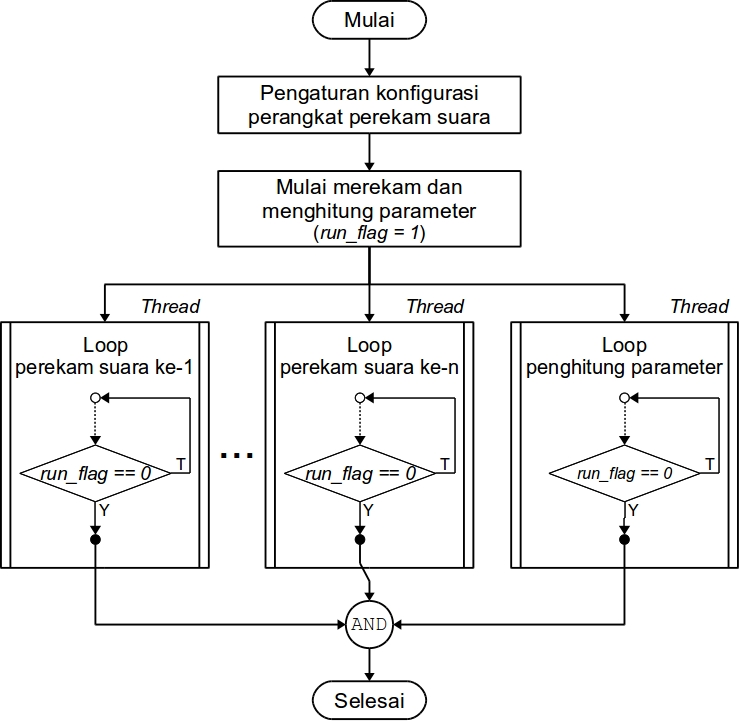
\includegraphics[scale=.5,keepaspectratio=true]{images/flowchart_main_wxspeacaltrain.jpg}
 \caption[Diagram alir SpeaCalTrain]{Diagram alir SpeaCalTrain.}
 \label{fig:flowchart_main_wxspeacaltrain}
\vskip .5em
\end{figure}

\begin{figure}[htp!]
\vskip 1em
\centering
 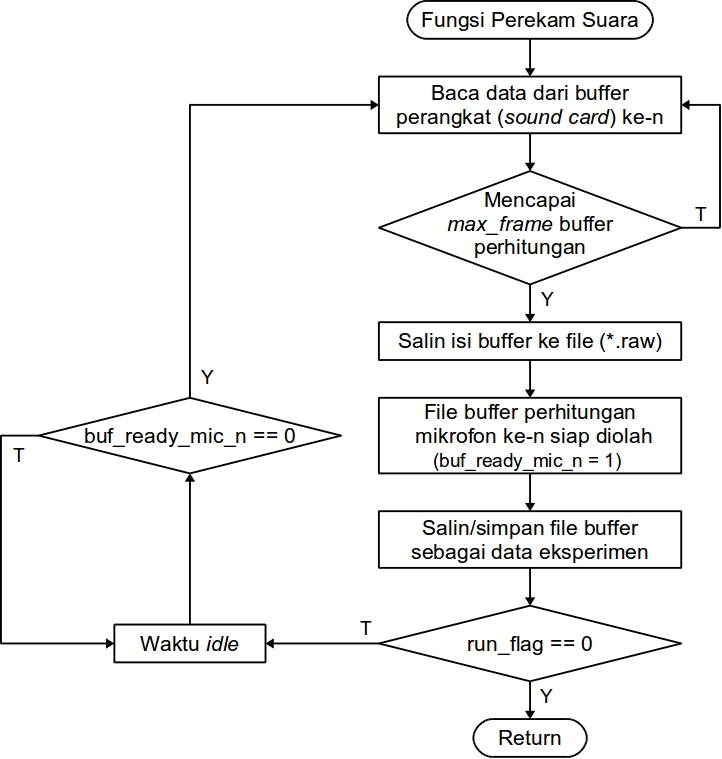
\includegraphics[scale=.5,keepaspectratio=true]{images/flowchart_record_wxspeacaltrain.jpg}
 \caption[Diagram alir fungsi perekam suara pada SpeaCalTrain]{Diagram alir fungsi perekam suara pada SpeaCalTrain.}
 \label{fig:flowchart_record_wxspeacaltrain}
\vskip .5em
\end{figure}

\begin{figure}[htp!]
\vskip 1em
\centering
 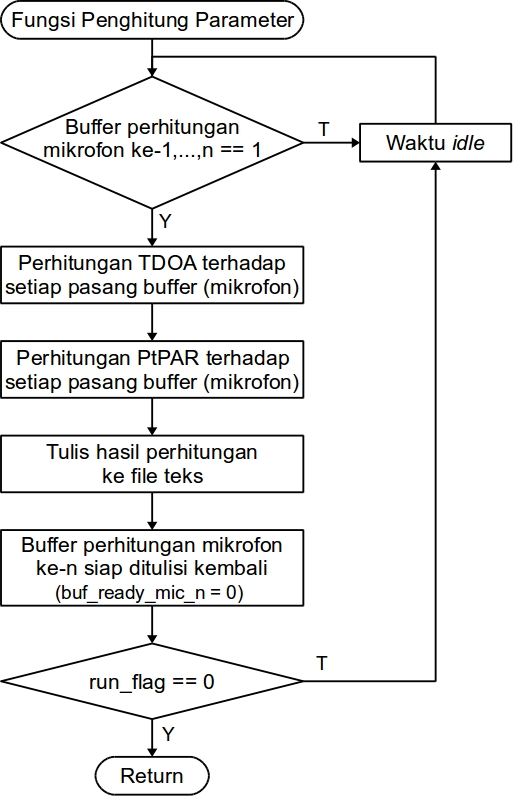
\includegraphics[scale=.5,keepaspectratio=true]{images/flowchart_compute_wxspeacaltrain.jpg}
 \caption[Diagram alir fungsi penghitung parameter TDOA dan PtPAR pada SpeaCalTrain]{Diagram alir fungsi penghitung parameter TDOA dan PtPAR pada SpeaCalTrain.}
 \label{fig:flowchart_compute_wxspeacaltrain}
\vskip .5em
\end{figure}

\begin{figure}[htp!]
\vskip 1em
\centering
 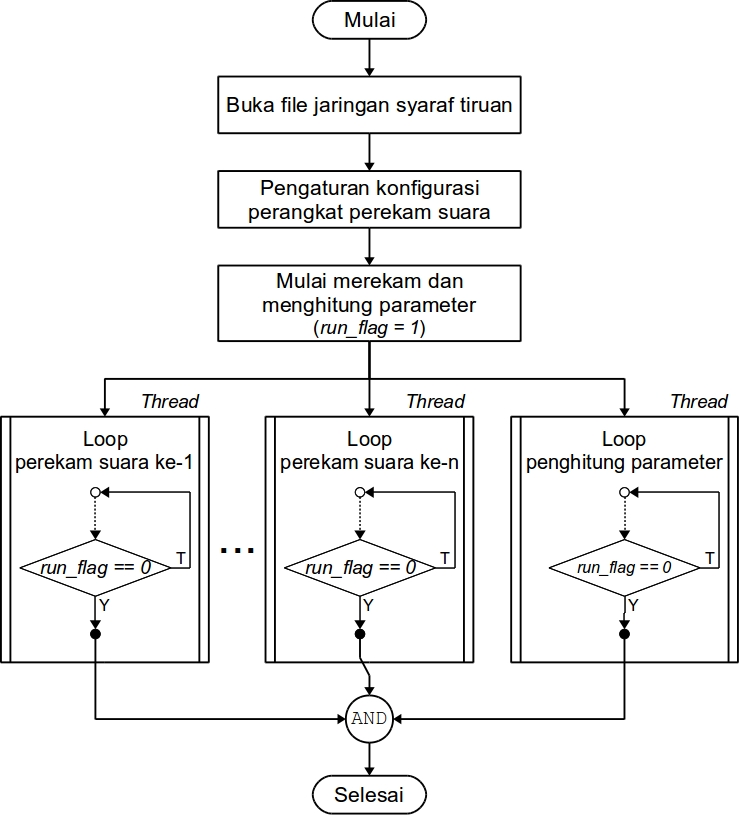
\includegraphics[scale=.5,keepaspectratio=true]{images/flowchart_main_wxspeacal.jpg}
 \caption[Diagram alir SpeaCal]{Diagram alir SpeaCal.}
 \label{fig:flowchart_main_wxspeacal}
\vskip .5em
\end{figure}

\begin{figure}[htp!]
\vskip 1em
\centering
 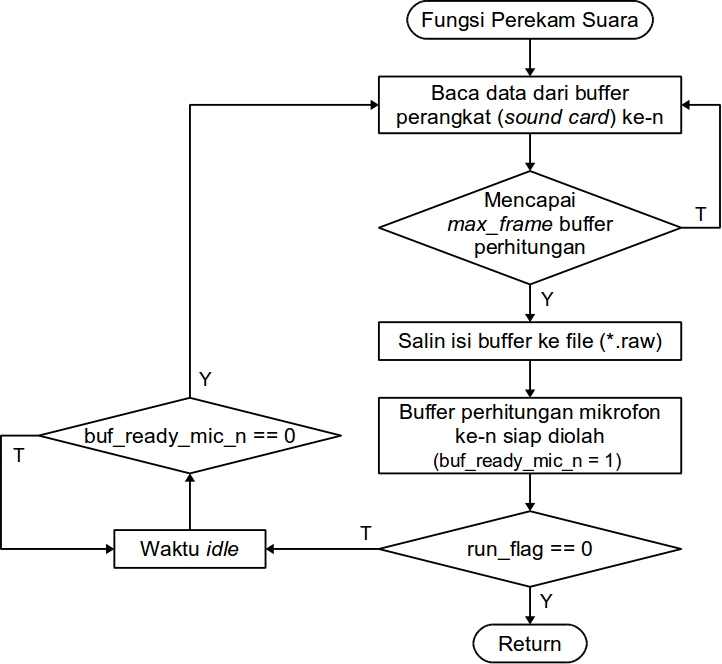
\includegraphics[scale=.5,keepaspectratio=true]{images/flowchart_record_wxspeacal.jpg}
 \caption[Diagram alir fungsi perekam suara pada SpeaCal]{Diagram alir fungsi perekam suara pada SpeaCal.}
 \label{fig:flowchart_record_wxspeacal}
\vskip .5em
\end{figure}

\begin{figure}[htp!]
\vskip 1em
\centering
 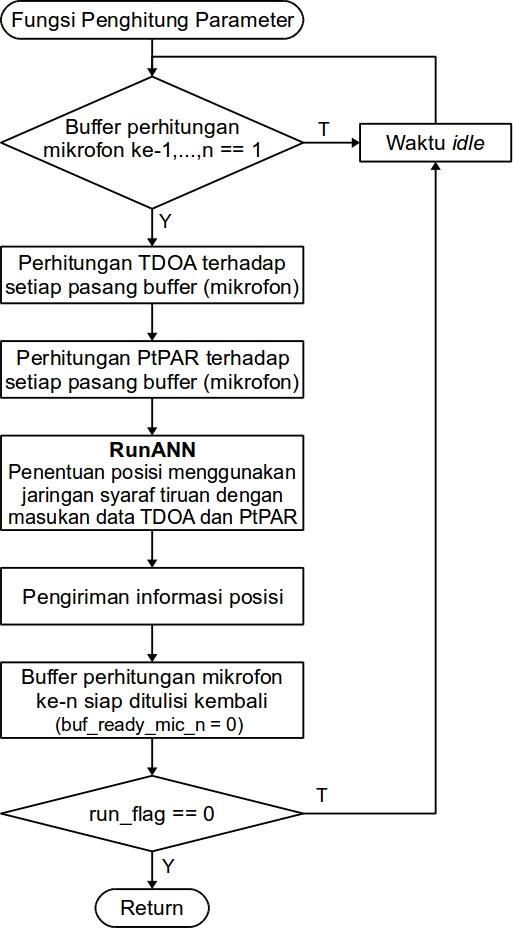
\includegraphics[scale=.5,keepaspectratio=true]{images/flowchart_compute_wxspeacal.jpg}
 \caption[Diagram alir fungsi penghitung parameter TDOA dan PtPAR pada SpeaCal]{Diagram alir fungsi penghitung parameter TDOA dan PtPAR pada SpeaCal.}
 \label{fig:flowchart_compute_wxspeacal}
\vskip .5em
\end{figure}

\begin{figure}[ht!]
\vskip 1em
\centering
 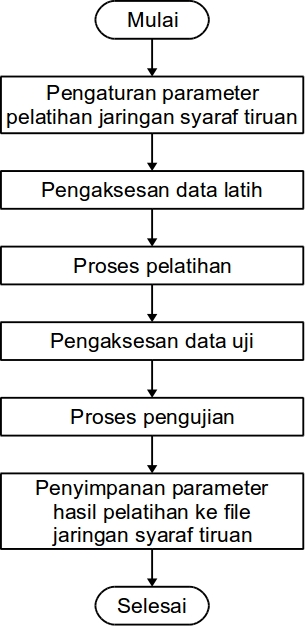
\includegraphics[scale=.5,keepaspectratio=true]{images/flowchart_main_anntraining.jpg}
 \caption[Diagram alir program untuk melatih JST]{Diagram alir program untuk melatih JST.}
 \label{fig:flowchart_main_anntraining}
\vskip .5em
\end{figure}


\subsubsection{Perangkat Keras}

Dalam penentuan posisi pengguna berdasarkan TDOA dan PtPAR, penempatan mikrofon akan sangat berpengaruh. Empat mikrofon yang digunakan akan ditempatkan pada perangkat \textit{multitouch} vertikal seperti yang ditunjukkan oleh \autoref{fig:desain_mic_1}. Dengan desain tersebut diharapkan posisi pengguna dalam ruang dapat diperkirakan. Apabila manusia dapat memperkirakan \textit{azimuth} posisi sumber suara dengan dua telinga, secara logis \textit{azimuth} posisi pengguna dapat diperkirakan dengan membandingkan sinyal yang tertangkap oleh mikrofon kanan dan kiri, sedangkan \textit{elevation} dapat diperkirakan dengan sinyal dari mikrofon atas dan bawah. Selain itu, dengan adanya perbedaan jarak mikrofon kanan-kiri dan mikrofon atas-bawah terhadap permukaan layar, diharapkan jarak pengguna terhadap layar juga dapat diperkirakan memanfaatkan parameter TDOA dan PtPAR yang membandingkan kombinasi mikrofon kanan-kiri dan mikrofon atas-bawah, misalnya parameter TDOA dan PtPAR pasangan mikrofon atas dan kanan. meskipun demikian, prioritas utama adalah memperolah \textit{azimuth} posisi pengguna relatif terhadap perangkat \textit{multitouch}.

\addtocontents{lof}{\vspace{4em} \hfill {Halaman} \par}

\begin{figure}[ht!]
\vskip 1em
  \begin{center}
    \subfigure[Tampak muka]
    {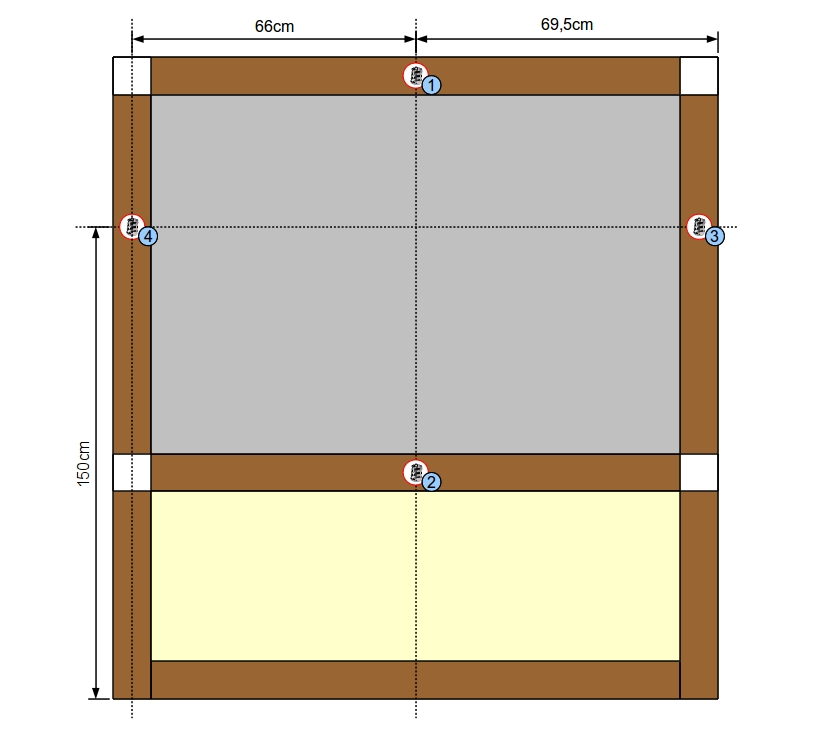
\includegraphics[scale=.5,keepaspectratio=true]{images/desain_mic_1a.jpg}
    \label{fig:desain_mic_1a}}
    \subfigure[Tampak atas]
    {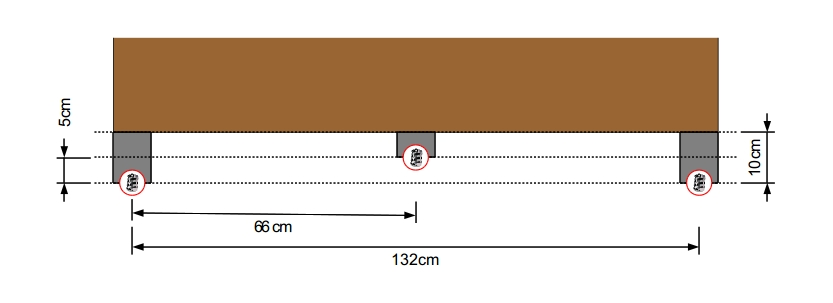
\includegraphics[scale=.5,keepaspectratio=true]{images/desain_mic_1b.jpg}
    \label{fig:desain_mic_1b}}
  \end{center}
  \caption[Rancangan penempatan mikrofon]{Rancangan penempatan mikrofon.}
  \label{fig:desain_mic_1}
  \vskip .5em
\end{figure}


\subsubsection{Pengambilan Data}

Pengambilan data latih dan uji untuk JST dilakukan dengan menempatkan sumber suara (\textit{speaker}) pada koordinat tertentu relatif terhadap perangkat \textit{multitouch} vertikal. Titik 0 dari koordinat Cartesian yang digunakan adalah ujung kiri atas perangkat \textit{multitouch}. Pengguna diasumsikan merupakan manusia dewasa dengan tinggi 160-170 cm. Dengan demikian, dapat diasumsikan bahwa posisi mulut berada pada ketinggian 150 cm dari tanah. Oleh karena itu, sumber suara ditempatkan pada koordinat $z = -30$, sedangkan koordinat $x$ dan $y$ merupakan variabel. Jangkauan nilai kedua koordinat tersebut adalah $x = \{-50, 10, 70, 130, 190\}$ dan $y = \{60, 120, 180\}$ (ditandai dengan tanda X pada \autoref{fig:floor_plan_1}).

\begin{figure}[ht!]
\vskip 1em
\centering
 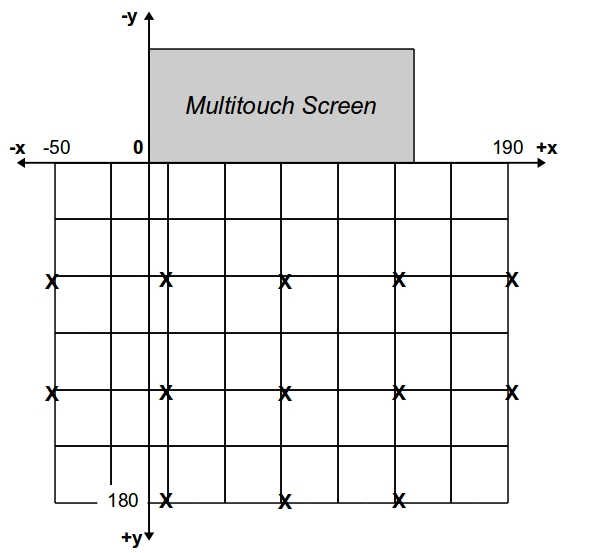
\includegraphics[scale=.5,keepaspectratio=true]{images/floor_plan_1.jpg}
 \caption[Rancangan titik pengambilan data]{Rancangan titik pengambilan data.}
 \label{fig:floor_plan_1}
\vskip .5em
\end{figure}


\subsection{Iterasi I: Implementasi}

\subsubsection{Perangkat Lunak}

Implementasi fungsi perekam suara memanfaatkan pustaka Portaudio untuk mengakses \textit{buffer} yang dimiliki \textit{sound card} dan menyalinnya ke sebuah file yang berekstensi \texttt{raw}. File-file yang berisi representasi sinyal suara dari empat mikrofon inilah yang kemudian akan diolah oleh fungsi penghitung parameter.

\singlespacing
\begin{figure}[htp!]
\vskip 1em
\begin{lstlisting}
if(inputBuffer == NULL)
{
	for(i=0; i<framesPerBuffer; i++)
    {
		output_data_buffer[i] = SAMPLE_SILENCE;  /* left */
		if(NUM_CHANNELS == 2)
			output_data_buffer[i] = SAMPLE_SILENCE;  /* right */
	}
}
else
{
	for(i=0; i<framesPerBuffer; i++)
	{
		output_data_buffer[i] = *input++;
	}
}
\end{lstlisting}
\caption[Kode program operasi pembacaan data dari \textit{buffer} yang dimiliki \textit{sound card}]{Kode program operasi pembacaan data dari \textit{buffer} yang dimiliki \textit{sound card}.}
\label{lst:read_sound_card_buffer}
\vskip .5em
\end{figure}
\onehalfspacing

\singlespacing
\begin{figure}[htp!]
\vskip 1em
\begin{lstlisting}
sprintf(recordFileName,"dev-%d-buf-rec-%d.raw", userDataFile->devNum, pubBufFileID);
buf_fid = fopen(recordFileName, "wb");
if(buf_fid == NULL)
{
	printf("Could not open file for saving the buffer.");
	exit(1);
}
else
{
	fwrite(output_data_buffer, NUM_CHANNELS * sizeof(SAMPLE), framesPerBuffer, buf_fid);
	fclose(buf_fid);
}
\end{lstlisting}
\caption[Kode program operasi penyimpanan data ke file yang berekstensi \texttt{raw}]{Kode program operasi penyimpanan data ke file yang berekstensi \texttt{raw}.}
\label{lst:save_data_to_raw_file}
\vskip .5em
\end{figure}
\onehalfspacing


Fungsi penghitung parameter terdiri dari penghitung parameter TDOA dan PtPAR. Metode CCC digunakan untuk menghitung TDOA dari sepasang data sinyal. Untuk memperoleh operasi yang cepat, metode CCC diimplentasikan menggunakan DFT. Oleh karena itu, fungsi ini memanfaatkan pustaka FFTW3 dalam proses penghitungan TDOA. \autoref{lst:ccc_op} menunjukkan implementasi metode CCC. Parameter TDOA dapat diperoleh dengan mencari nilai maksimum dari hasil operasi CCC.

\singlespacing
\begin{figure}[htp!]
\vskip 1em
\begin{lstlisting}
pa = fftw_plan_dft_1d((N << 1) - 1, signala_ext, outa, FFTW_FORWARD, FFTW_ESTIMATE);
pb = fftw_plan_dft_1d((N << 1) - 1, signalb_ext, outb, FFTW_FORWARD, FFTW_ESTIMATE);
px = fftw_plan_dft_1d((N << 1) - 1, out, out_shifted, FFTW_BACKWARD, FFTW_ESTIMATE);

for (i = 0; i < (N << 1) - 1; i++) {
	if (i < N) {
		signala_ext[i] = signala[i];
		signalb_ext[i] = signalb[i];
	}
	else {
		signala_ext[i] = 0;
		signalb_ext[i] = 0;
	}
}

fftw_execute(pa);
fftw_execute(pb);

for (i = 0; i < (N << 1) - 1; i++)
	out[i] = outa[i] * conj(outb[i]);

fftw_execute(px);

for (i = 0; i < (N << 1) - 1; i++)
	result[i] = out_shifted[(i + N) % ((N << 1) - 1)] / ((N << 1) - 1);
\end{lstlisting}
\caption[Kode program operasi CCC terhadap dua data sinyal]{Kode program operasi CCC terhadap dua data sinyal.}
\label{lst:ccc_op}
\vskip .5em
\end{figure}
\onehalfspacing


\singlespacing
\begin{figure}[htp!]
\vskip 1em
\begin{lstlisting}
maxTemp1 = minTemp1 = creal(first_xcorr_signal[0]);;
maxTemp2 = minTemp2 = creal(second_xcorr_signal[0]);

for(l = 0; l < FramesPerBuffer; l++) {
	if(creal(first_xcorr_signal[l]) > maxTemp1)
		maxTemp1 = creal(first_xcorr_signal[l]);
	if(creal(first_xcorr_signal[l]) < minTemp1)
		minTemp1 = creal(first_xcorr_signal[l]);
	if(creal(second_xcorr_signal[l]) > maxTemp2)
		maxTemp2 = creal(second_xcorr_signal[l]);
	if(creal(second_xcorr_signal[l]) < minTemp2)
		minTemp2 = creal(second_xcorr_signal[l]);
}

return 20*log10((maxTemp1-minTemp1)/(maxTemp2-minTemp2));
\end{lstlisting}
\caption[Kode program operasi perhitungan PtPAR]{Kode program operasi perhitungan PtPAR.}
\label{lst:ptpar_op}
\vskip .5em
\end{figure}
\onehalfspacing


\subsubsection{Perangkat Keras}

Implementasi rancangan penempatan mikrofon dapat dilihat pada \autoref{fig:desain_mic_1c}. Mikrofon ditancapkan pada \textit{styrofoam} yang ditempelkan pada perangkat \textit{multitouch} vertikal (\autoref{fig:desain_mic_2c2}). Selain sebagai tempat untuk meletakkan mikrofon, \textit{styrofoam} juga dapat berfungsi sebagai peredam suara. Oleh karena itu, diharapkan mikrofon hanya menangkap sinyal suara dari arah depan.

\begin{figure}[ht!]
\vskip 1em
\centering
 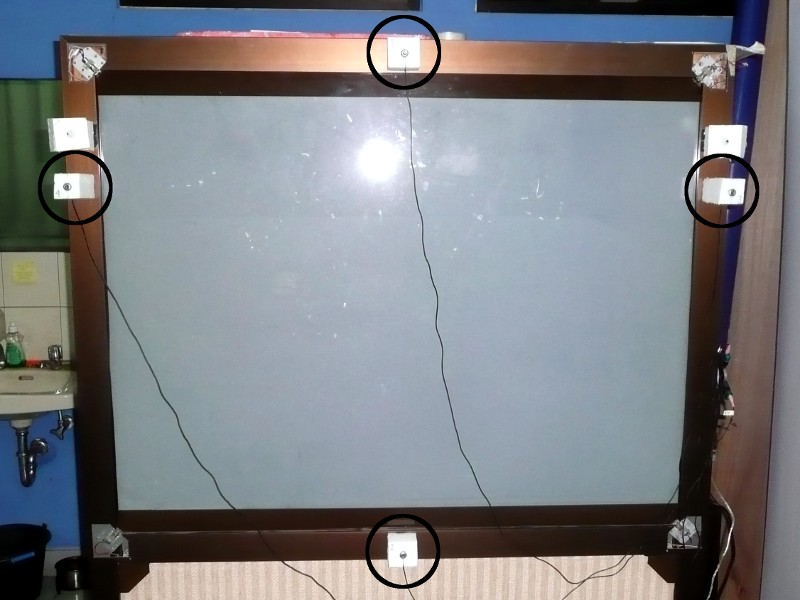
\includegraphics[width=.9\textwidth,keepaspectratio=true]{images/desain_mic_1c.jpg}
 \caption[Foto implementasi rancangan penempatan mikrofon]{Foto implementasi rancangan penempatan mikrofon.}
 \label{fig:desain_mic_1c}
\vskip .5em
\end{figure}


\subsection{Iterasi I: Pengujian dan Evaluasi}

Pengambilan data dilakukan dengan memutar secara berulang-ulang file rekaman suara FAN\_1A dan MAA\_1A yang berisi ucapan kata "satu". Masing-masing rekaman menghasilkan sebuah set data yang memuat 78 data dari 13 titik pengambilan data yang telah didefinisikan pada \autoref{subsec:iter1_desain} (6 data per titik). \autoref{fig:1_fan_1a_34}  dan \autoref{fig:1_maa_1a_34} menunjukkan parameter TDOA dan PtPAR pasangan mikrofon 3 dan 4 dari set data FAN\_1A dan MAA\_1A. Untuk memudahkan pembacaan grafik, jangkauan nilai koordinat $x = \{-50, 10, 70, 130, 190\}$ dan $y = \{60, 120, 180\}$ diubah menjadi $x = \{-2, -1, 0, 1, 2\}$ dan $y = \{-1, 0, 1\}$.

Grafik-grafik dari dua set data tersebut memperlihatkan bahwa nilai parameter PtPAR tidak cukup konsisten dan nilai parameter TDOA sangat tidak konsisten. Dua set data ini tidak dapat digunakan untuk  melatih JST yang baik.

\begin{figure}[htp!]
\vskip 1em
  \begin{center}
    \subfigure[PtPAR]
    {\fbox{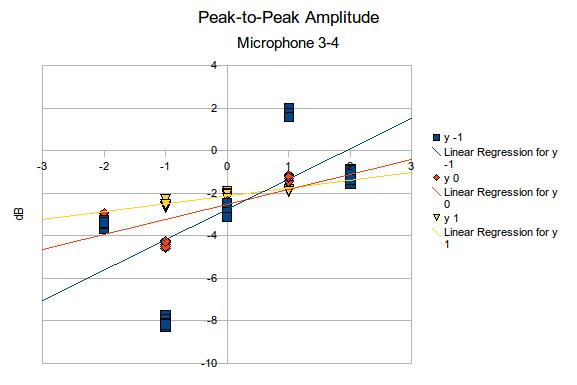
\includegraphics[scale=.55,keepaspectratio=true]{images/1_ptpar_fan_1a_34.jpg}
    \label{fig:1_ptpar_fan_1a_34}}}
    \subfigure[TDOA]
    {\fbox{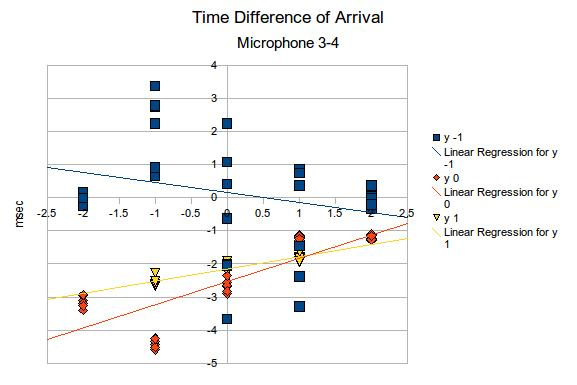
\includegraphics[scale=.55,keepaspectratio=true]{images/1_tdoa_fan_1a_34.jpg}
    \label{fig:1_tdoa_fan_1a_34}}}
  \end{center}
  \caption[Grafik TDOA dan PtPAR mikrofon 3-4 dari set data FAN\_1A]{Grafik TDOA dan PtPAR mikrofon 3-4 dari set data FAN\_1A.}
  \label{fig:1_fan_1a_34}
  \vskip .5em
\end{figure}

\begin{figure}[htp!]
\vskip 1em
  \begin{center}
    \subfigure[PtPAR]
    {\fbox{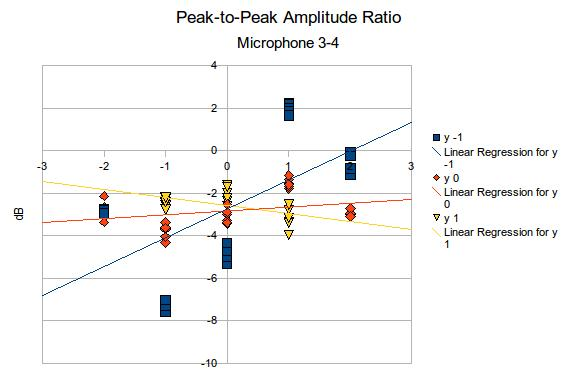
\includegraphics[scale=.55,keepaspectratio=true]{images/1_ptpar_maa_1a_34.jpg}
    \label{fig:1_ptpar_maa_1a_34}}}
    \subfigure[TDOA]
    {\fbox{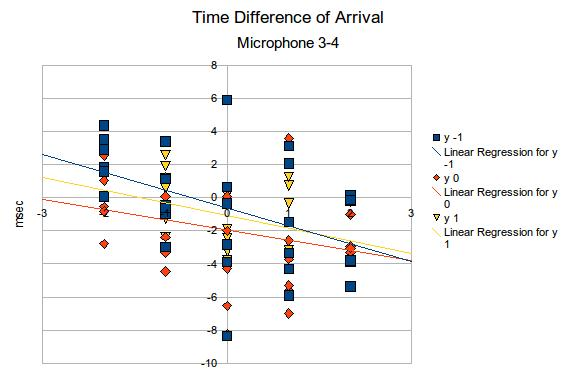
\includegraphics[scale=.55,keepaspectratio=true]{images/1_tdoa_maa_1a_34.jpg}
    \label{fig:1_tdoa_maa_1a_34}}}
  \end{center}
  \caption[Grafik TDOA dan PtPAR mikrofon 3-4 dari set data MAA\_1A]{Grafik TDOA dan PtPAR mikrofon 3-4 dari set data MAA\_1A.}
  \label{fig:1_maa_1a_34}
  \vskip .5em
\end{figure}
